\section{Partie 2 : Drone}
    \subsection{Drone : Généralités}
        \begin{frame}[allowframebreaks]{Drone : Généralités}
            \begin{columns}[T]
                \begin{column}{0.5\textwidth}
                    \begin{exampleblock}{}
                        \begin{itemize}
                            \item Marque DJI - ancien modèle plus actif en production
                            \item Conçu pour les développeurs
                            \item Nombreux tutoriels
                            \item Applications possibles diverses
                                \begin{itemize}
                                    \item Applications Android/iOS
                                    \item Applications sur ordinateurs embarqués
                                \end{itemize}
                        \end{itemize}
                    \end{exampleblock}
                \end{column}\hfill
                \begin{column}{0.5\textwidth}
                    \begin{figure}
                        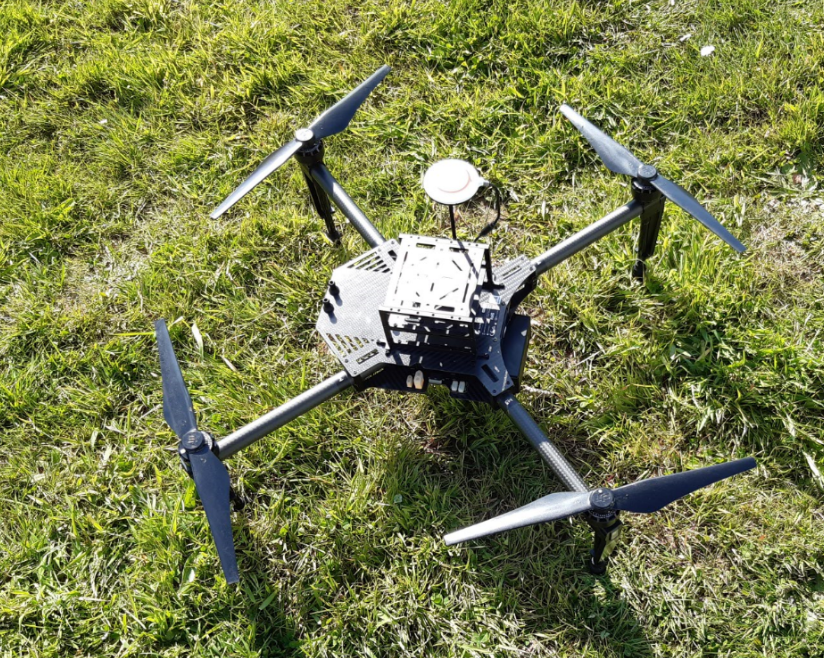
\includegraphics[width=1\linewidth]{images/drone.png}
                        \caption*{Matrice 100 - Vue aérienne}
                    \end{figure}
                \end{column}
            \end{columns}
        \end{frame}
%
% ---------------------------------------------------------------- %
        \begin{frame}[allowframebreaks]
                \begin{block}{}
                    \begin{itemize}
                        \setbeamertemplate{itemize item}[square]
                        \item Équipements nécessaires
                            \begin{itemize}
                                \item Ordinateur embarqué : Raspberry Pi 3B+ (avec alimentation et carte SD 32Go)
                                \item Caméra Raspberry Pi v2.1
                            \end{itemize}
                        \item Installation du SDK fourni par DJI
                        \item Communication via le port série
                    \end{itemize}
                \end{block}
            \end{frame}
%
% ---------------------------------------------------------------- %
    \subsection{Drone : Architecture finale}
        \begin{frame}[allowframebreaks]
            \begin{figure}[H]
    			\centering
    			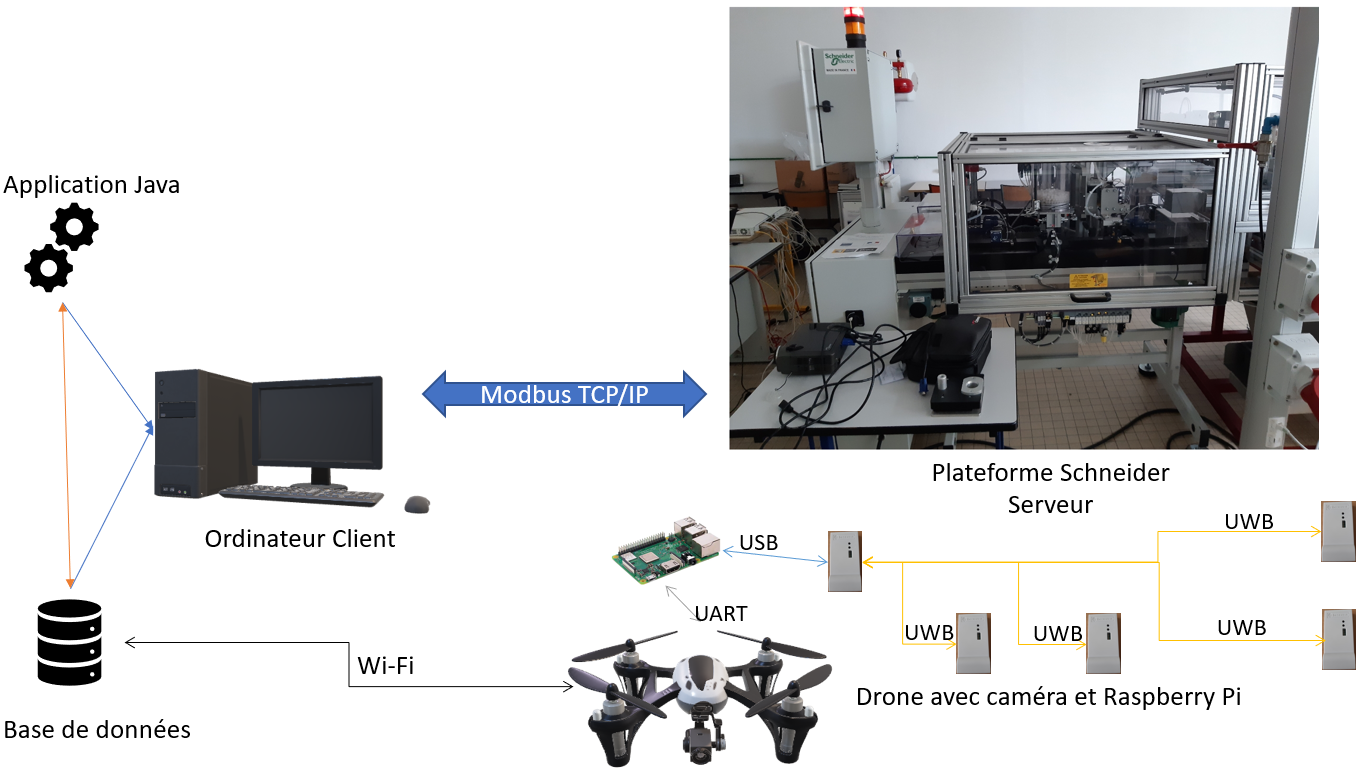
\includegraphics[width=0.9\linewidth]{images/architectureGeneraleTotale.png}
    			\label{fig:archiGen}
    		\end{figure}
        \end{frame}
%
% ---------------------------------------------------------------- %
    \subsection{Drone : Positionnement}
            \begin{frame}[allowframebreaks]{Drone : Positionnement}
                \begin{columns}
                    \begin{column}{0.5\textwidth}
                        \begin{block}{}
                            \begin{itemize}
                                \setbeamertemplate{itemize item}[square]
                                \item Positionnement GPS impossible : utilisation en intérieure du drone
                                \item Utilisation de cartes Decawave
                                \item Protocole de communication UWB
                                \item Une carte accrochée sur le drone (tag)
                                \item 4 cartes connectées dans la pièce (ancre)
                            \end{itemize}
                        \end{block}
                    \end{column}\hfill
                    \begin{column}{0.5\textwidth}
                        \begin{figure}[H]
                            \centering
                            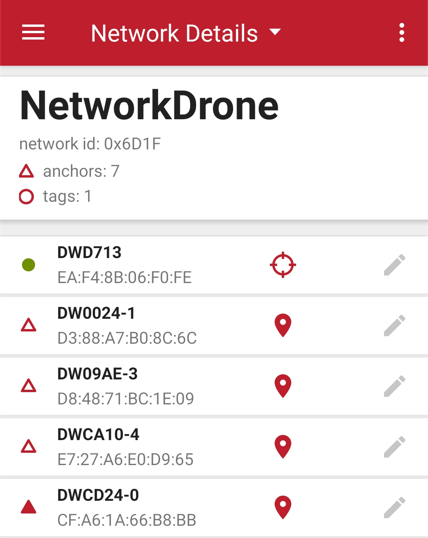
\includegraphics[width=0.9\linewidth]{images/UI_Decawave1.png}
                            \caption*{}
                        \end{figure}
                    \end{column}
                \end{columns}
            \end{frame}
%
% ---------------------------------------------------------------- %
            %\begin{frame}[allowframebreaks]
             %   \begin{figure}[H]
        	%		\centering
        	%		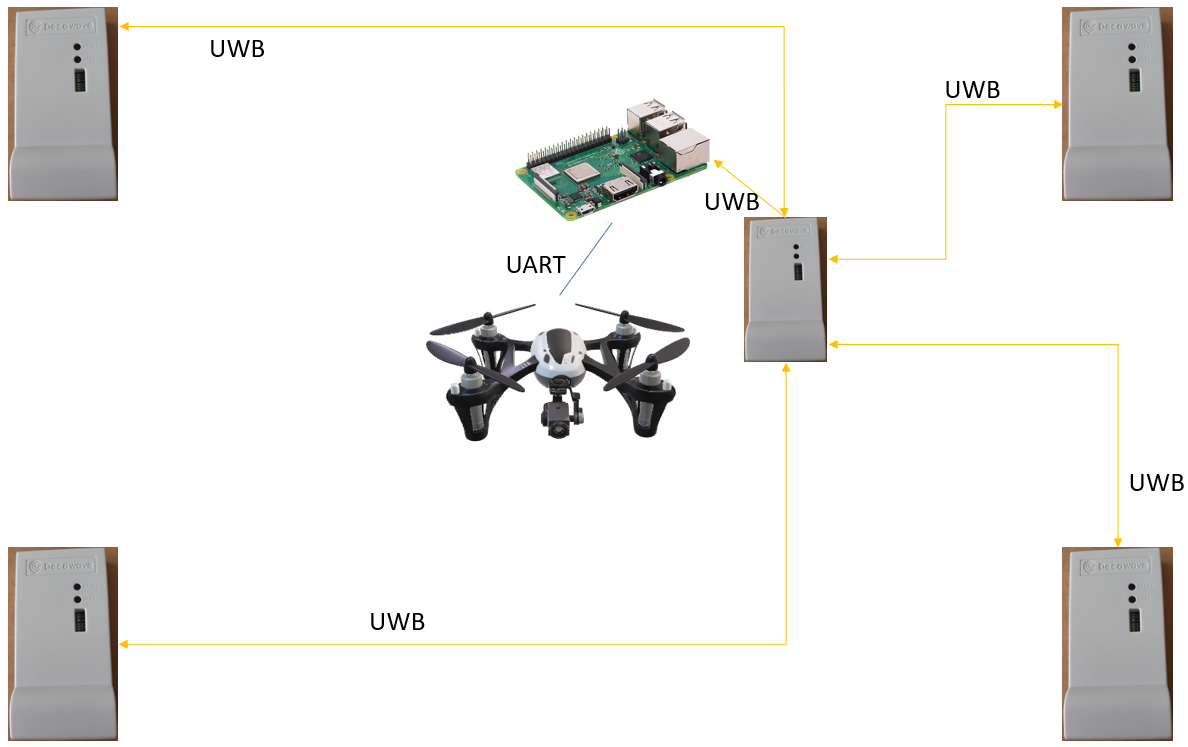
\includegraphics[width=0.9\linewidth]{images/architectureDrone.png}
        	%		\label{fig:archiDrone}
        	%	\end{figure}
            %\end{frame}
%
% ---------------------------------------------------------------- %
            \begin{frame}[allowframebreaks]
                % possibilité d'ajouter Bancroft et Newton
                \begin{block}{}
                    \begin{itemize}
                        \setbeamertemplate{itemize item}[square]
                        \item 2 méthodes testées : Bancroft et Newton/Raphson
                        \item Test de Bancroft avec 5 et 7 ancres connectées
                    \end{itemize}
                \end{block}
                
                \begin{table}[H]
                    \resizebox{\textwidth}{!}{
                        \begin{tabular}{| c | c | c |}
                            \hline
                            \textbf{Méthode} & \textbf{Temps d'exécution} & \textbf{Valeur du vecteur résultat} \\[0.15cm] \hline
                            Réalité & / & 0.76 0.43 0.26 \\[0.15cm]
                            \hline
                            Bancroft 7 ancres & entre 520 µs et 1200 µs & 0.71 0.80 0.78 \\[0.15cm]
                            \hline
                            Bancroft 5 ancres & entre 450 µs et 1200 µs & 0.68 1.37 1.46 \\[0.15cm]
                            \hline
                        \end{tabular}
                    }
                    \caption*{Résultats obtenus avec 5 et 7 ancres sur le positionnement avec Bancroft}
                \end{table}
            \end{frame}
%
% ---------------------------------------------------------------- %
            \begin{frame}[allowframebreaks]
                \begin{block}{}
                    \begin{itemize}
                        \setbeamertemplate{itemize item}[square]
                        \item Résultats avec Bancroft très médiocres
                        \item Limité à 4 ancres pour le calcul de la position (Decawave)
                    \end{itemize}
                \end{block}
                
                \begin{table}[H]
                \resizebox{\textwidth}{!}{
                    \begin{tabular}{| c | c | c | c |}
                        \hline
                        \textbf{Méthode} & \textbf{Temps d'exécution} & \textbf{Valeur du vecteur résultat} & \textbf{RSME} \\[0.15cm] \hline
                        Réalité & / & 0.76 0.43 0.26 & / \\[0.15cm]
                        \hline
                        Bancroft & $\cong$ 840 µs & 0.98 -0.11 0.35 & 0.34 \\[0.15cm]
                        \hline
                        Decawave & $\cong$ 840 µs & 0.78 0.38 0.26 & 0.07 \\[0.15cm]
                        \hline
                    \end{tabular}
                }
                \caption*{\label{table:resAll}Comparaisons des résultats obtenus avec Bancroft et Decawave}
            \end{table}
            \end{frame}
%
% ---------------------------------------------------------------- %
        \subsection{Drone : Déplacement}
            \begin{frame}[allowframebreaks]{Drone : Déplacement}
                \begin{figure}[H]
        			\centering
        			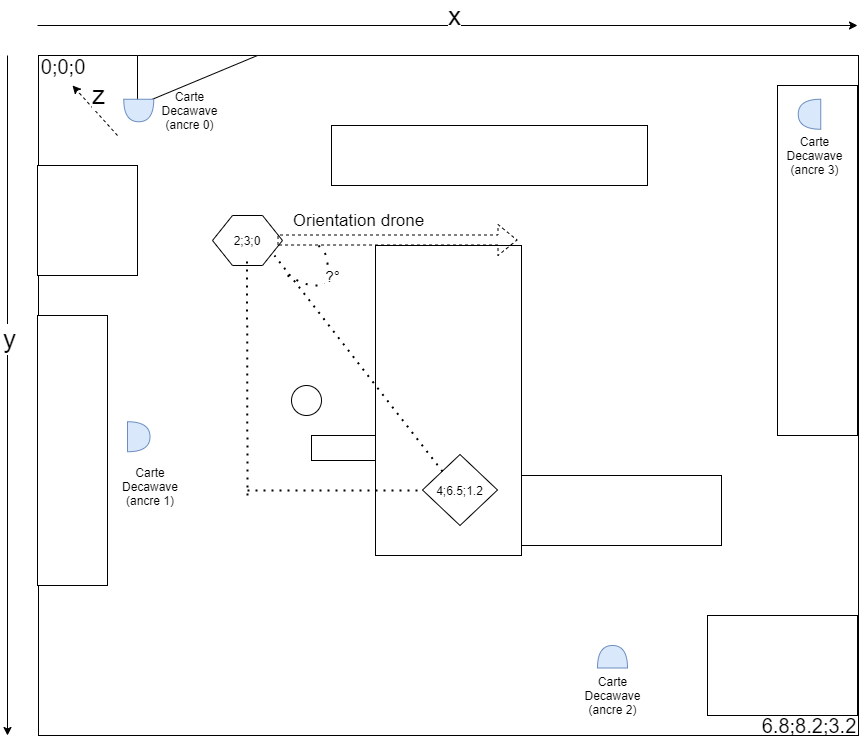
\includegraphics[width=0.67\linewidth]{images/methodologie.png}
        		\end{figure}
        		
        		
        		\begin{columns}
                    \begin{column}{0.5\textwidth}
                        \begin{block}{}
                            \begin{itemize}
                                \setbeamertemplate{itemize item}[square]
                                \item Pas d'accès direct à la valeur de la boussole
                                \item Absence de fonction dans le SDK afin de récupérer la valeur directement
                                \item Contraint de passer par une valeur détournée
                            \end{itemize}
                        \end{block}
                    \end{column}\hfill
                    \begin{column}{0.5\textwidth}
                        \begin{figure}[H]
                            \centering
                            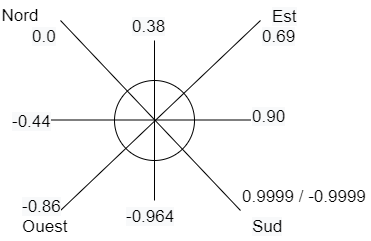
\includegraphics[width=1\linewidth]{images/roseVents.png}
                        \end{figure}
                    \end{column}
                \end{columns}
                
                \begin{figure}[H]
                    \centering
                    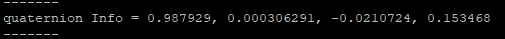
\includegraphics[width=1\linewidth]{images/quat.png}
                \end{figure}
            \end{frame}
%
% ---------------------------------------------------------------- %
    %\subsection{Drone : Architecture finale}
    %    \begin{frame}[allowframebreaks]
     %       \begin{figure}[H]
    %			\centering
    %			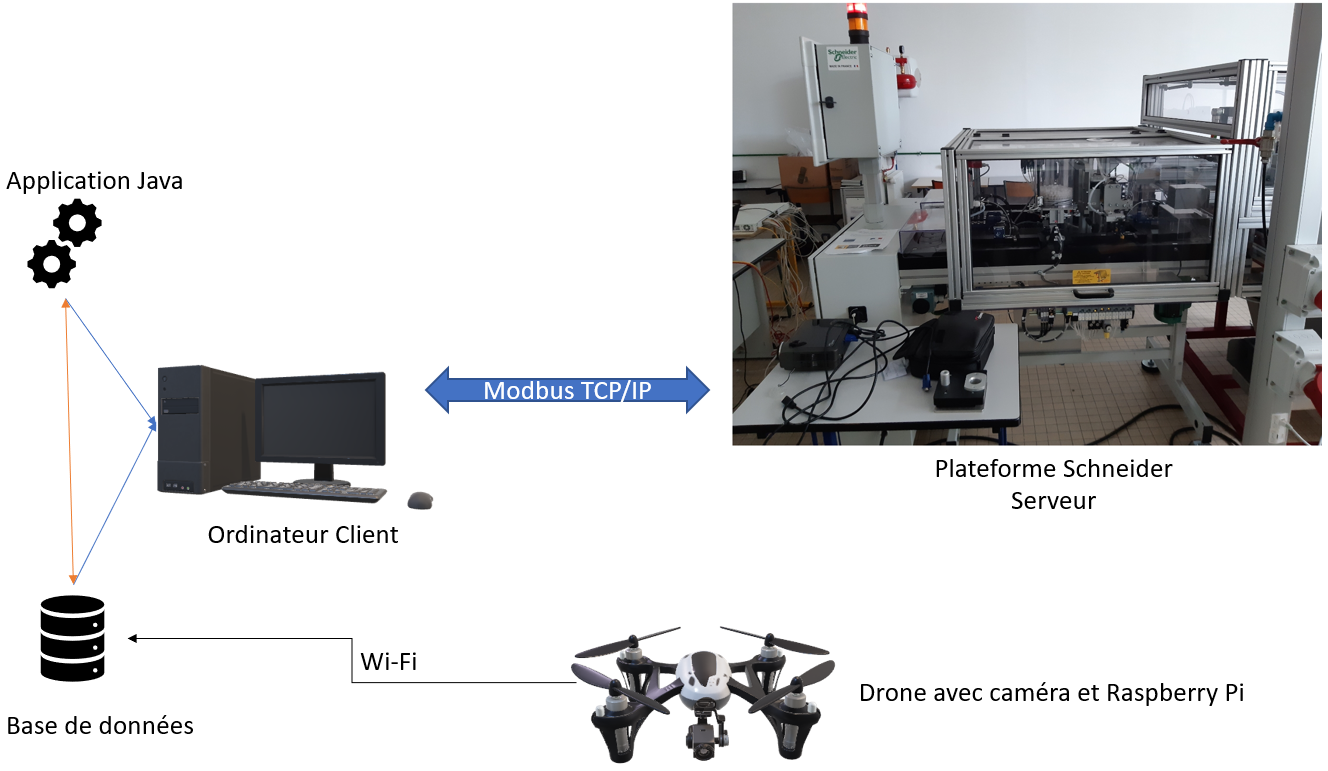
\includegraphics[width=0.9\linewidth]{images/architectureGenerale.png}
    %			\label{fig:archiGen}
    %		\end{figure}
    %    \end{frame}
%
% ---------------------------------------------------------------- %